\documentclass{beamer}
\usepackage[utf8]{inputenc}

\usetheme{Madrid}
\usecolortheme{default}
\usepackage{amsmath,amssymb,amsfonts,amsthm}
\usepackage{txfonts}
\usepackage{tkz-euclide}
\usepackage{listings}
\usepackage{adjustbox}
\usepackage{array}
\usepackage{tabularx}
\usepackage{gvv}
\usepackage{lmodern}
\usepackage{circuitikz}
\usepackage{tikz}
\usepackage{graphicx}

\setbeamertemplate{page number in head/foot}[totalframenumber]

\usepackage{tcolorbox}
\tcbuselibrary{minted,breakable,xparse,skins}



\definecolor{bg}{gray}{0.95}
\DeclareTCBListing{mintedbox}{O{}m!O{}}{%
  breakable=true,
  listing engine=minted,
  listing only,
  minted language=#2,
  minted style=default,
  minted options={%
    linenos,
    gobble=0,
    breaklines=true,
    breakafter=,,
    fontsize=\small,
    numbersep=8pt,
    #1},
  boxsep=0pt,
  left skip=0pt,
  right skip=0pt,
  left=25pt,
  right=0pt,
  top=3pt,
  bottom=3pt,
  arc=5pt,
  leftrule=0pt,
  rightrule=0pt,
  bottomrule=2pt,
  toprule=2pt,
  colback=bg,
  colframe=orange!70,
  enhanced,
  overlay={%
    \begin{tcbclipinterior}
    \fill[orange!20!white] (frame.south west) rectangle ([xshift=20pt]frame.north west);
    \end{tcbclipinterior}},
  #3,
}
\lstset{
    language=C,
    basicstyle=\ttfamily\small,
    keywordstyle=\color{blue},
    stringstyle=\color{orange},
    commentstyle=\color{green!60!black},
    numbers=left,
    numberstyle=\tiny\color{gray},
    breaklines=true,
    showstringspaces=false,
}
%------------------------------------------------------------
%This block of code defines the information to appear in the
%Title page
\title %optional
{2.8.39}
\date{}
%\subtitle{A short story}

\author % (optional)
{Sai Krishna Bakki - EE25BTECH11049}

\begin{document}
\frame{\titlepage}
\begin{frame}{Question}
Find the angle between the lines whose direction cosines are given by the equations
 $l+m+n=0$, $l^2+m^2-n^2=0$.
\end{frame}
\begin{frame}{Setting Up the Equations in Matrix Form}

We begin by representing the given system of equations using vectors and matrices. Let the direction cosines be represented by the column vector $\vec{x}$:
\begin{align}
\vec{x} = \myvec{l\\m\\n}
\end{align}
The three conditions on the direction cosines can be written in matrix form:
\begin{align}
 l + m + n = 0 \implies \vec{C}^T \vec{x} = 0, \vec{C} = \myvec{1\\1\\1}
 \end{align}
 \begin{align}
     l^2 + m^2 - n^2 = 0 \implies \vec{x}^T \vec{A} \vec{x} = 0, \vec{A} = \myvec{ 1 & 0 & 0 \\ 0 & 1 & 0 \\ 0 & 0 & -1 }
     \end{align}
     \end{frame}
\begin{frame}{Setting Up the Equations in Matrix Form}
     \begin{align}
     l^2 + m^2 + n^2 = 1 \implies \vec{x}^T \vec{I} \vec{x} = 1, \vec{I}=  \myvec{ 1 & 0 & 0 \\ 0 & 1 & 0 \\ 0 & 0 & 1 }
     \end{align}
\end{frame}
\begin{frame}{Solving for the Direction Cosine Vectors}
    Our goal is to find the two vectors, $\vec{D}_1$ and $\vec{D}_2$, that satisfy these matrix equations.
 We can efficiently find the value of $n$ by subtracting the two quadratic form equations:
\begin{align}
\vec{x}^T \vec{I} \vec{x} - \vec{x}^T \vec{A} \vec{x} = 1 \implies \vec{x}^T (\vec{I} - \vec{A}) \vec{x} = 1
\end{align}
The matrix $(\vec{I} - \vec{A})$ is:
\begin{align}
\vec{I} - \vec{A} = \myvec{ 1 & 0 & 0 \\ 0 & 1 & 0 \\ 0 & 0 & 1 } -\myvec{ 1 & 0 & 0 \\ 0 & 1 & 0 \\ 0 & 0 & -1 } = \myvec{ 0 & 0 & 0 \\ 0 & 0 & 0 \\ 0 & 0 & 2 }
\end{align}
Substituting this back into the equation (0.5) gives:
\begin{align}
\myvec{ l & m & n } \myvec{ 0 & 0 & 0 \\ 0 & 0 & 0 \\ 0 & 0 & 2} \myvec{ l \\ m \\ n} = 1
\end{align}
\begin{align}
2n^2 = 1 \implies n = \pm \frac{1}{\sqrt{2}}
\end{align}
    
\end{frame}
\begin{frame}{Solving for the Direction Cosine Vectors}
    Let's choose $n = -\frac{1}{\sqrt{2}}$. Substituting this into the remaining linear and normalization equations gives a system for $l$ and $m$:
\begin{align}
     \myvec{1&1&1}\myvec{l\\ m \\ \frac{-1}{\sqrt{2}}}=0 \implies l+m=\frac{1}{\sqrt{2}}
     \end{align}
     \begin{align}
     % l^2 + m^2 + \left(-\frac{1}{\sqrt{2}}\right)^2 = 1 \implies l^2 + m^2 = \frac{1}{2}
     \myvec{l &m &\frac{-1}{\sqrt{2}}}\myvec{ 1 & 0 & 0 \\ 0 & 1 & 0 \\ 0 & 0 & 1 }\myvec{l &m &\frac{-1}{\sqrt{2}}} \implies l^2 + m^2 = \frac{1}{2}
     \end{align}
     
Squaring the first part gives
\begin{align}
(l+m)^2 = \left(\frac{1}{\sqrt{2}}\right)^2 \implies l^2+2lm+m^2 = \frac{1}{2}
\end{align}

subsituting equation (0.10) in equation (0.11),we get
\begin{align}
    2lm=0
\end{align}
so we get l=0 and m=0,
\begin{align}
      l=0, m = \frac{1}{\sqrt{2}};
      m=0,l = \frac{1}{\sqrt{2}}
\end{align}
\end{frame}
\begin{frame}{Assembling the Direction Cosine Vectors}
    Combining our results, the two direction cosine vectors are:
\begin{align}    
\vec{D}_1 = \myvec{ 0 \\ \frac{1}{\sqrt{2}} \\ \frac{-1}{\sqrt{2}} } \quad \text{and} \quad \vec{D}_2 = \myvec{ \frac{1}{\sqrt{2}} \\ 0 \\ \frac{-1}{\sqrt{2}}}
\end{align}
\end{frame}

\begin{frame}{Calculating the Angle Between the Direction Cosines}
    The cosine of the angle $\theta$ between the lines is the dot product of their direction cosine vectors. Using matrix multiplication, this is 
\begin{align}
\cos \theta = \vec{D}_1^T \vec{D}_2\\ 
\cos \theta = \myvec{ 0 & \frac{1}{\sqrt{2}} & \frac{-1}{\sqrt{2}}} \myvec{ \frac{1}{\sqrt{2}} \\ 0 \\ \frac{-1}{\sqrt{2}} }
\end{align}


\begin{align}
\cos \theta = 0 + 0 + \frac{1}{2} = \frac{1}{2}
\end{align}
Therefore, the angle is:
\begin{align}
\theta = cos^{-1}\brak{\frac{1}{2}} = 60^{\circ} \quad \text{or} \quad \frac{\pi}{3} \text{ radians}
\end{align}
\end{frame}

\begin{frame}[fragile]
\frametitle{C Code }
\begin{lstlisting}
#include <math.h>

#ifndef M_PI
#define M_PI 3.14159265358979323846
#endif

/* --- Helper Function --- */
// Calculates the Euclidean norm (magnitude) of a 3D vector.
static inline double calculate_norm(const double vec[3]) {
    return sqrt(vec[0] * vec[0] + vec[1] * vec[1] + vec[2] * vec[2]);
}

/* --- Core Logic Function --- */
// This function is "exported" so it can be called from other programs.
#ifdef __cplusplus
extern "C" {
#endif

\end{lstlisting}
\end{frame}  
\begin{frame}[fragile]
\frametitle{C Code }
\begin{lstlisting}
double get_angle_between_lines() {
    // Direction ratios derived from solving the system of equations.
    double d1_ratios[] = {0.0, 1.0, -1.0};
    double d2_ratios[] = {1.0, 0.0, -1.0};
    double d1_cosines[3], d2_cosines[3];

    // Calculate the magnitude (norm) of each direction ratio vector.
    double norm_d1 = calculate_norm(d1_ratios);
    double norm_d2 = calculate_norm(d2_ratios);

    // Calculate the direction cosines by normalizing the vectors.
    for (int i = 0; i < 3; ++i) {
        d1_cosines[i] = d1_ratios[i] / norm_d1;
        d2_cosines[i] = d2_ratios[i] / norm_d2;
    }
\end{lstlisting}
\end{frame}  
\begin{frame}[fragile]
\frametitle{C Code }
\begin{lstlisting}
    // Calculate the dot product of the two direction cosine vectors.
    double cos_theta = 0.0;
    for (int i = 0; i < 3; ++i) {
        cos_theta += d1_cosines[i] * d2_cosines[i];
    }
    
    // Calculate the angle in radians and convert to degrees.
    double angle_rad = acos(cos_theta);
    return angle_rad * (180.0 / M_PI);
}

#ifdef __cplusplus
}
#endif
\end{lstlisting}
\end{frame}  
\begin{frame}[fragile]
\frametitle{Python Code through Shared Output}
\begin{lstlisting}
# Code by GVV Sharma
# July 22, 2024
# Released under GNU GPL
# This script finds the angle between two lines by calling a standard C shared library.

import numpy as np
import matplotlib.pyplot as plt
from mpl_toolkits.mplot3d import Axes3D
import ctypes
import os
# --- Load the C Shared Library using ctypes ---
try:
    # Construct the full path to the library file, assuming it's in the same directory.
    lib_path = os.path.join(os.path.dirname(os.path.abspath(__file__)), 'angle_calculator_lib.so')
   angle_lib = ctypes.CDLL(lib_path)

    \end{lstlisting}
\end{frame}  
\begin{frame}[fragile]
\frametitle{Python Code through Shared Output}
\begin{lstlisting}
except OSError:
    print("Error: 'angle_calculator_lib.so' not found.")
    print("Please compile the C library by running this command in your terminal:")
    print("gcc -shared -o angle_calculator_lib.so -fPIC angle_calculator_lib.c")
    exit()
# --- Define the function signature from the C library ---
# Tell ctypes that the function returns a C double. This is crucial for correctness.
angle_lib.get_angle_between_lines.restype = ctypes.c_double

# --- Call the C function ---
angle_deg = angle_lib.get_angle_between_lines()
angle_rad = np.deg2rad(angle_deg)
# --- For Plotting Purposes (re-defining vectors in Python) --
# Direction ratios
d1_ratios = np.array([0, 1, -1])
d2_ratios = np.array([1, 0, -1])
\end{lstlisting}
\end{frame}  
\begin{frame}[fragile]
\frametitle{Python Code through Shared Output}
\begin{lstlisting}
# Direction cosines (unit vectors)
d1 = d1_ratios / np.linalg.norm(d1_ratios)
d2 = d2_ratios / np.linalg.norm(d2_ratios)

print("--- Calculation performed by standard C library via ctypes ---")
print(f"The angle between the lines is {angle_rad:.4f} radians.")
print(f"The angle between the lines is {angle_deg:.2f} degrees.")
print("-" * 55)


# --- Plotting the vectors in 3D ---
fig = plt.figure(figsize=(8, 8))
ax = fig.add_subplot(111, projection='3d')

# Origin point
origin = [0, 0, 0]
\end{lstlisting}
\end{frame}  
\begin{frame}[fragile]
\frametitle{Python Code through Shared Output}
\begin{lstlisting}
# Plot the direction cosine vectors
label1 = f'Line 1 DC: ({d1[0]:.2f}, {d1[1]:.2f}, {d1[2]:.2f})'
label2 = f'Line 2 DC: ({d2[0]:.2f}, {d2[1]:.2f}, {d2[2]:.2f})'
ax.quiver(*origin, *d1, color='r', label=label1)
ax.quiver(*origin, *d2, color='b', label=label2)

# Set plot limits
ax.set_xlim([-1.5, 1.5])
ax.set_ylim([-1.5, 1.5])
ax.set_zlim([-1.5, 1.5])

# Add labels and title
ax.set_xlabel('X axis')
ax.set_ylabel('Y axis')
ax.set_zlabel('Z axis')
ax.set_title('Visualization of the Two Lines in 3D (Angle from C Library)')
ax.legend()
\end{lstlisting}
\end{frame}  
\begin{frame}[fragile]
\frametitle{Python Code through Shared Output}
\begin{lstlisting}
ax.grid(True)

# Equal aspect ratio
ax.set_box_aspect([1,1,1])

plt.show()
\end{lstlisting}
\end{frame}  
\begin{frame}[fragile]
\frametitle{Python Code }
\begin{lstlisting}
# Code by GVV Sharma
# July 22, 2024
# Released under GNU GPL
# This script finds the angle between two lines whose direction cosines
# are given by the equations:

import numpy as np
import matplotlib.pyplot as plt
from mpl_toolkits.mplot3d import Axes3D

# From the mathematical derivation, we found the direction ratios for the two lines.
# Case 1 (l=0) gives direction ratios proportional to (0, 1, -1)
d1_ratios = np.array([0, 1, -1])

# Case 2 (m=0) gives direction ratios proportional to (1, 0, -1)
d2_ratios = np.array([1, 0, -1])

\end{lstlisting}
\end{frame}  
\begin{frame}[fragile]
\frametitle{Python Code }
\begin{lstlisting}
print(f"Direction ratios for Line 1: {d1_ratios}")
print(f"Direction ratios for Line 2: {d2_ratios}")
print("-" * 30)

# --- Calculate Direction Cosines ---
# To get the direction cosines, we normalize the direction ratio vectors (divide by their magnitude).
norm_d1 = np.linalg.norm(d1_ratios)
norm_d2 = np.linalg.norm(d2_ratios)

# The direction cosines are the components of the unit vectors.
d1 = d1_ratios / norm_d1
d2 = d2_ratios / norm_d2

print(f"Direction cosines for Line 1: [{d1[0]:.4f}, {d1[1]:.4f}, {d1[2]:.4f}]")
print(f"Direction cosines for Line 2: [{d2[0]:.4f}, {d2[1]:.4f}, {d2[2]:.4f}]")
print("-" * 30)

\end{lstlisting}
\end{frame}  
\begin{frame}[fragile]
\frametitle{Python Code }
\begin{lstlisting}
# --- Calculate the angle using the dot product of direction cosines ---
# The dot product of two unit vectors (direction cosines) is the cosine of the angle between them.
cos_theta = np.dot(d1, d2)

# Calculate the angle in radians
angle_rad = np.arccos(cos_theta)

# Convert the angle to degrees
angle_deg = np.degrees(angle_rad)

print(f"Cosine of the angle (from dot product of cosines): {cos_theta:.4f}")
print("-" * 30)
print(f"The angle between the lines is {angle_rad:.4f} radians.")
print(f"The angle between the lines is {angle_deg:.2f} degrees.")

\end{lstlisting}
\end{frame}  
\begin{frame}[fragile]
\frametitle{Python Code }
\begin{lstlisting}
# --- Plotting the vectors in 3D ---
fig = plt.figure(figsize=(8, 8))
ax = fig.add_subplot(111, projection='3d')

# Origin point
origin = [0, 0, 0]
print(f"The angle between the lines is {angle_rad:.4f} radians.")
print(f"The angle between the lines is {angle_deg:.2f} degrees.")

# Plot the direction cosine vectors (unit vectors) as arrows from the origin
label1 = f'Line 1 DC: ({d1[0]:.2f}, {d1[1]:.2f}, {d1[2]:.2f})'
label2 = f'Line 2 DC: ({d2[0]:.2f}, {d2[1]:.2f}, {d2[2]:.2f})'
ax.quiver(*origin, *d1, color='r', label=label1)
ax.quiver(*origin, *d2, color='b', label=label2)

\end{lstlisting}
\end{frame}  
\begin{frame}[fragile]
\frametitle{Python Code }
\begin{lstlisting}
# Set the plot limits to be consistent
ax.set_xlim([-1.5, 1.5])
ax.set_ylim([-1.5, 1.5])
ax.set_zlim([-1.5, 1.5])

# Add labels and title
ax.set_xlabel('X axis')
ax.set_ylabel('Y axis')
ax.set_zlabel('Z axis')
ax.set_title('Visualization of the Two Lines in 3D')
ax.legend()
ax.grid(True)

# To make the aspect ratio equal
ax.set_box_aspect([1,1,1]) 

# Show the plot
plt.show()

\end{lstlisting}
\end{frame}  
\begin{frame}{Plot By C code and Python Code}
    \begin{figure}
    \centering
    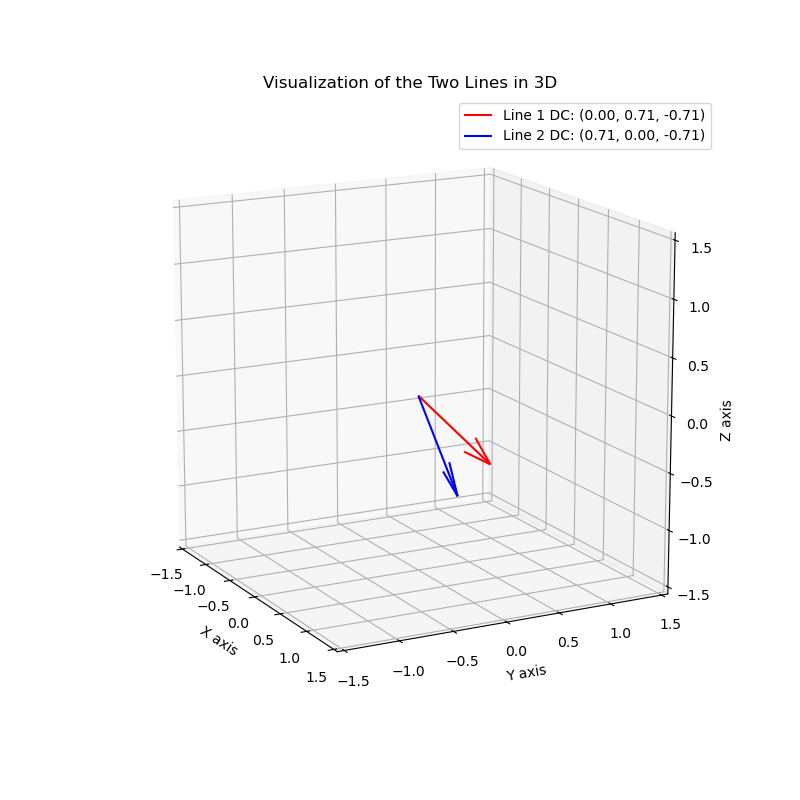
\includegraphics[width=0.7\columnwidth]{figs/Figure_1.png}
    \label{fig:placeholder}
\end{figure}
\end{frame}
\end{document}
